\section{Architettura Front-End} \label{sec:archfront}
L'intera applicazione è stata sviluppata in React. La scelta di tale tecnologia ha portato l'interfaccia grafica ad essere sviluppata in componenti, composti tra di loro fino a configurare la GUI finale.\\
Per ricercare una modularità del codice, così da aumentare la leggibilità e la manutenibilità dello stesso, sono stati creati più componenti per ogni pagina, che interagiscono e si compongono tra di loro, fino a costituire la pagina finale. Questo approccio, tipico di React e dei pattern adottati per il front-end, permette di suddividere il codice, evitando che esso venga inserito interamente nella singola pagina.\\
L'interfaccia utente prevede due pagine, definite dalle due macro funzionalità dell'applicazione. Una pagina è dedicata alla gestione della documentazione, l'altra all'interazione con il chatbot.\\
Gli elementi comuni alle due pagine principali sono stati implementati con uguali componenti, così da riutilizzare il codice ove possibile, senza dover ridefinire gli stessi elementi grafici più volte.\\ \\
Nella descrizione della architettura che costituisce il front-end dell'applicazione, sarà riportato un UML delle componenti principali di ogni pagina e per ognuna di esse sarà riportata una descrizione dettagliata, con una lista degli elementi che la compongono e dei requisiti associati a tale componente.

\newpage

\subsection{Documents Page}

La Documents Page è la pagina relativa alla gestione della documentazione presente nell'applicazione. È possibile visualizzare quali sono i documenti che l'utente ha già inserito, le loro informazione, la form per effettuare l'upload di un nuovo documento e i bottoni per visualizzarli ed eliminarli.\\
È presente una sidebar a comparsa, comune a quello presente anche nella Chat Page, dove è posizionato il form per il caricamento dei documenti e dove è possibile modificare le impostazioni dell'applicazione.

\begin{figure}[h!]
    \centering  
    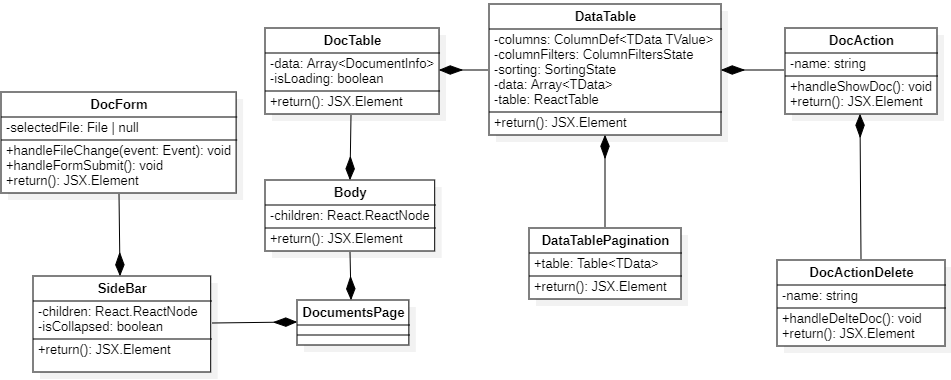
\includegraphics[width=\textwidth]{DocumentPageView.png}
    \caption{UML dei componenti principali della Documents Page}
\end{figure}

\subsubsection{SideBar}

\textbf{Descrizione}\\
Questo componente costituisce il menù a tendina comune alle due pagine dell'applicazione. In esso è presente il componente Settings, dove tramite ModelToggle e ThemeToggle è possibile cambiare il LLM e il tema utilizzato dall'applicazione.\\
Oltre alle impostazioni generali dell'applicativo, in questo componente viene posizionato il DocForm utilizzato per caricare nuovi componenti nel sistema.\\ \\
\textbf{Elementi}\\
Il valore booleano isCollapsed è gestito dallo stato del componente, e determina se mostrare o meno il menù a comparsa. La modifica di questo valore è associato all'evento onClick di un bottone.\\
Il componente Settings, nel quale sono inseriti i due componenti Toggle, è costituito da un Dialog che mostra il suo contenuto mediante l'azione di un DialogTrigger. In questo modo, ModelToggle e ThemeToggle sono renderizzati solo a seguito dell'interazione con il pulsante del menù.\\
All'interno di questi due componenti Toggle, viene impostato il tema e il modello da utilizzare modificando un valore controllato dallo stato dei componenti stessi.\\ \\
\textbf{Requisiti associati}
\begin{itemize}[itemsep=-4pt]
    \item RFO-1;
    \item RFO-2.
\end{itemize}

\subsubsection{Body}

\textbf{Descrizione}\\
Il componente Body rappresenta il corpo della pagina. In esso sono inseriti tutti i componenti necessari alla visualizzazione dei documenti dell'applicazione, contenuti da DocTable.\\ \\
\textbf{Elementi}\\
Al suo interno è contenuto il solo componente DocTable.

\subsubsection{DocForm}

\textbf{Descrizione}\\
Conenuto all'interno della Sidebar, DocForm è il componente che contiene la form con cui effettuare l'upload di nuovi documenti nel sistema. Qui grazie ad un Input è possibile selezionare il documento di interesse ed inviarlo grazie ad un apposito bottone.\\ \\
\textbf{Elementi}\\
Grazie ad un componente Input che permette la selezione di soli file con estensione .pdf, .docx e .mp3, è possibile inviare un documento grazie ad un Button, a cui è associata la funzione handleFormSubmit tramite evento onClick. All'interno di questa funzione è verificato il valore di selectedFile, il quale viene utilizzato per fornire i dati necessari per effettuare le effettive operazioni per caricare il documento.\\
Per accertare il corretto formato del documento selezionato, viene utilizzata la funzione handleFileChange, invocata ogni qual volta viene utilizzato il form Input, che deseleziona ogni file con estensione diversa da quella aspettata, mostrando contestualmente un messaggio d'errore.\\ \\
\textbf{Requisiti associati}
\begin{itemize}[itemsep=-4pt]
    \item RFO-29;
    \item RFO-30;
    \item RFO-31;
    \item RFD-32;
    \item RFD-34;
    \item RFO-66;
    \item RFD-67;
    \item RFD-68;
    \item RFZ-69.
\end{itemize}

\subsubsection{DocTable}

\textbf{Descrizione}\\
La DocTable è il componente che definisce la tabella nella quale sono visualizzati i documenti presenti nell'applicazione.\\ \\
\textbf{Elementi}\\
Tramite l'utilizzo dello hook useEffect, ogni volta che viene cambiato il modello utilizzato dall'applicazione vengono recuperate le informazioni sui documenti presenti a sistema. Questi dati, definiti dall'interfaccia DocumentInfo e composti dal nome del documento (string), dalla data di inserimento a sistema (string), dalla dimensione (number) e dai tag assegnati (string), sono utilizzati per formare il componente DataTable che, costruendo la tabella, è responsabile di renderizzare la lista finale dei documenti.\\
Il valore booleano isLoading identifica se è in corso o meno l'operazione di recupero dei documenti. Esso viene utilizzato per renderizzare, internamente a DataTable, il componente IsLoadingDoc, che mostra un componente Skeleton momentaneo.

\subsubsection{DataTable}

\textbf{Descrizione}\\
È il componente responsabile della visualizzazione delle informazioni dei documenti. Oltre alla tabella, contiene i componenti responsabili alla ricerca, al filtraggio, alla visualizzazione e all'eliminazione dei documenti, oltre che a DataTablePagination e DataTableViewOption. Queste ultime sono utilizzate per gestire la logica di renderizzazione della tabella.\\ \\
\textbf{Elementi}\\
I dati che costituiscono la tabella sono inseriti all'interno di componenti adibiti a questo preciso ruolo, quali Table, TableBody, TableCell, TableHead, TableHeader e TableRow.\\
La tabella contiene in ogni sua riga le informazioni dei documenti presenti, oltre che le azioni sul documento (visualizzazione, eliminazione e cambio tag) tramite il componente DocAction.\\
La ricerca, effettuata tramite la digitazione su un componente Input, permette di mostrare i documenti in base al loro nome e data di inserimento, tramite una ricerca che agisce sulle string di nome e data, tramite un valore setFilterValue. La ricerca avviene per data (true) o per nome (false) in base al valore booleano della variabile setIsFilterData, che varia con un evento onClick di due componenti DropdownMenuItem.\\
I componenti DataTablePagination e DataTableViewOption, posti all'interno di DataTable, agiscono sulla paginazione della tabella.\\ \\
\textbf{Requisiti associati}
\begin{itemize}[itemsep=-4pt]
    \item RFO-3;
    \item RFO-4;
    \item RFO-5;
    \item RFO-6;
    \item RFZ-7;
    \item RFD-9;
    \item RFO-10;
    \item RFO-11;
    \item RFO-12;
    \item RFO-13.
\end{itemize}

\subsubsection{DataTablePagination e DataTableViewOption}

\textbf{Descrizione}\\
È il componente che gestisce la logica di renderizzazione della tabella, dividendo i dati della stessa in più pagine e permettendone la navigazione mediante pulsanti.\\ \\
\textbf{Elementi}\\
Tramite i componenti Select, SelectContent, SelectItem, SelectTrigger e SelectValue, DataTablePagination divide i dati presenti in tabella, così da mostrarne per pagina tanti quanti il valore di pageSize. Questo valore è stabilito dall'interazione con un componente Select, che agisce all'evento onValueChange chiamando setPageSize, funzione responsabile della modifica effettiva del valore numerico.\\
La navigazione nella tabella avviene con l'evento onClick di vari Button, che tramite le funzioni setPageIndex, previousPage e nextPage variano i dati da mostrare a schermo.\\
Nel componente DataTableViewOption, tramite un DropdownMenu contenente dei DropdownMenuCheckboxItem, è presente la logica che permette la renderizzazione delle sole colonne della tabella selezionate.

\subsubsection{DocAction}

\textbf{Descrizione}\\
La componente DocAction contiene tutti gli elementi necessari ad effettuare le azioni previste sui documenti, ovvero visualizzazione, eliminazione e cambio tag.\\ \\
\textbf{Elementi}\\
Grazie ad un menù a comparsa formato con i componenti DropdownMenu, DropdownMenuContent, DropdownMenuItem, DropdownMenuLabel, DropdownMenuSeparator e DropdownMenuTrigger, DocAction permette la visualizzazone del documento di interesse grazie all'evento onClick del DropdownMenuItem. Questo evento chiama la funzione handleShowDoc che, recuperato dal back-end l'url del documento, apre in modalità blank una nuova scheda del browser, dove poter visualizzare il documento.\\
L'azione di eliminazione è invece lasciata al componente DocActionDelete, contenuto da DocAction.\\ \\
\textbf{Requisiti associati}
\begin{itemize}[itemsep=-4pt]
    \item RFO-8;
    \item RFZ-15;
    \item RFZ-16;
    \item RFD-36;
    \item RFD-37.
\end{itemize}

\subsubsection{DocActionDelete}
\textbf{Descrizione}\\
È la componente responsabile della logica con cui l'utente può eliminare un documento.\\ \\
\textbf{Elementi}\\
Dall'interazione con un AlertDialogTrigger, viene aperto un AlertDialog per confermare l'eliminazione del documento dal sistema. All'evento onClick dell'AlertDialogAction, viene chiamata la funzione handleDelteDoc con cui viene richiesta al back-end l'eliminazione del documento e di ogni informazioni ad esso associata.\\ \\
\textbf{Requisiti associati}
\begin{itemize}[itemsep=-4pt]
    \item RFO-27;
    \item RFO-28.
\end{itemize}

\newpage

\subsection{Chat Page}
La Chat Page è la pagina relativa allo scambio di messaggi tra l'utente ed il chatbot integrato nell'applicazione. Nella schermata principale, è possibile visualizzare i messaggi inviati dall'utente, le risposte del chatbot, le fonti delle risposte e l'orario in cui sono stati inviati i messaggi. \\
È presente una sidebar laterale, nella quale sono presenti dei bottoni che permettono di visualizzare informazioni aggiuntive riguardanti le chat avviate in precedenza, un buttone per creare nuove chat, uno per eliminarle e un tasto con le impostazioni generali dell'applicazione, comune anche alla Documents Page.
\begin{figure}[h!]
    \centering  
    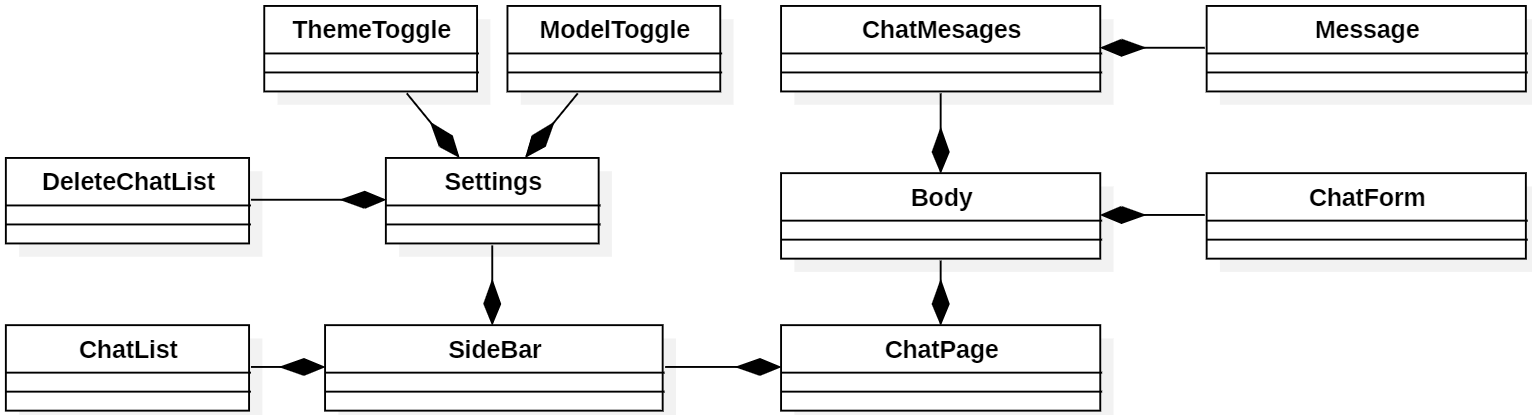
\includegraphics[width=\textwidth]{ChatPageView.png}
    \caption{UML dei componenti principali della Chat Page} 
\end{figure}

\subsubsection{SideBar}
\textbf{Descrizione}\\
Questo componente costituisce il menù a tendina comune alle due pagine dell’applicazione. In esso è presente il componente Settings, dove tramite ModelToggle e ThemeToggle è possibile cambiare il LLM e il tema utilizzato dall’applicazione. Con DeleteChatList è invece possibile eliminare tutte le conversazioni ancora attive.\\
Inoltre, tramite la ChatList, è possibile visualizzare la lista delle sessioni di chat effettuate e attive nel sistema, oltre ad un bottone per creare nuove chat.\\ \\
\textbf{Elementi}\\
La struttura della SideBar è identica a quella della DocumentPage. L'unica differenza riguarda i componenti presenti al suo interno.\\
Il componente Settings contenuto in SideBar, oltre ad aver ThemeToggle e ModelToggle, presenta DeleteChatList, adibito alla eliminazione di tutte le sessioni del sistema.\\
La lista delle sessioni è renderizzata tramite il componente ChatList, contenuto nella SideBar, che prende il posto del DocForm presente all'interno della Documents Page.
\\


\textbf{Requisiti associati}
\begin{itemize}[itemsep=-4pt]
    \item RFO-1;
    \item RFO-2.
\end{itemize}

\subsubsection{Body}

\textbf{Descrizione}\\
Il componente Body rappresenta il corpo della pagina. In esso sono inseriti tutti i componenti necessari alla visualizzazione dell'area di chat, contenuti da ChatForm e ChatMessages.\\ \\
\textbf{Elementi}\\
Al suo interno sono presenti i componenti ChatForm e ChatMessages.

\subsubsection{ChatList}
\textbf{Descrizione}\\
Il componente ChatList è la parte dell'interfaccia utente responsabile della gestione e visualizzazione delle sessioni di chat, consentendo agli utenti di selezionare, creare ed eliminare sessioni di chat, e fornendo un feedback visivo durante il caricamento dei dati.\\ \\
\textbf{Elementi}\\
Il componente ChatList utilizza l'hook useChatsData per gestire i dati delle chat e fornisce funzionalità per la creazione e l'eliminazione di chat. L'elenco delle chat è mostrato all'interno di un'area scrollabile, con opzioni per eliminare le chat esistenti. Quando viene eliminata una chat, lo stato viene aggiornato per riflettere la modifica.\\
ChatList è composta da una serie di elementi Button, i quali rappresentano  le chat avviate in precedenza nell'applicazione. Tramite funzioni asincrone, se i bottoni vengono cliccati allora verranno evidenziati, andando ad indicare quale chat sta venendo visualizzata nella sezione centrale della pagina. Per ciascun bottone, è inserito lateralmente un ulteriore bottone, il quale una volta cliccato, fa apparire un DropDownMenu, composto da DropDownMenuTrigger, DropDownMenuContent, DropDownMenuLabel, DropDownMenuSeparator. La voce del menù è un ulteriore bottone che permette la cancellazione della singola chat.  \\ \\
\textbf{Requisiti associati}
\begin{itemize}[itemsep=-4pt]
    \item RFD-48;
    \item RFD-49;
    \item RFO-53;
    \item RFO-54.
\end{itemize}

\subsubsection{DeleteChatList}
\textbf{Descrizione}\\
Il componente DeleteChatList fornisce un'interfaccia utente per eliminare tutte le sessioni di chat all'interno dell'applicazione, inclusa una finestra di dialogo di conferma, la gestione delle azioni e l'aggiornamento della sezione laterale dei threads al momento della cancellazione riuscita.\\ \\
\textbf{Elementi}\\
Il componente utilizza l'hook useChatsData per gestire lo stato delle chat e il componente AlertDialog per confermare l'azione di eliminazione. Quando l'utente conferma l'eliminazione, la funzione handleDeleteAllChat viene chiamata per eseguire l'operazione e aggiornare lo stato della chat. In caso di errore, viene visualizzato un messaggio.\\ \\
\textbf{Requisiti associati}
\begin{itemize}[itemsep=-4pt]
    \item RFD-50;
    \item RFD-51.
\end{itemize}

\subsubsection{ChatForm}
\textbf{Descrizione}\\
Questa componente è responsabile della raccolta dell'input dell'utente per i messaggi di chat, della validazione dell'input, della gestione dei dati della sessione di chat e dell'invio dei messaggi al server.\\ \\
\textbf{Elementi}\\
Il componente ChatForm utilizza l'hook useForm di react-hook-form per gestire lo stato e la validazione del form, insieme a due altri hook per gestire i dati dei messaggi e delle chat. Il form include un campo di testo per l'input del messaggio e un pulsante di invio. Quando l'utente invia il messaggio, il componente gestisce la validazione, l'invio dei dati e la visualizzazione di eventuali errori tramite un messaggio di errore. \\ \\
\textbf{Requisiti associati}
\begin{itemize}[itemsep=-4pt]
    \item RFO-40;
    \item RFO-41.
\end{itemize}

\subsubsection{ChatMessages e Message}
\textbf{Descrizione}\\
Il componente ChatMessages è responsabile della visualizzazione dei messaggi all'interno di una sessione di chat, differenziando tra i messaggi generati dall'utente e quelli generati dall'intelligenza artificiale, gestendo la visualizzazione dei messaggi quando non ce ne sono, e fornendo una Scroll Area per una navigazione agevole attraverso la cronologia della chat.\\ \\
\textbf{Elementi}\\
Sfruttando l'hook useMessagesData, il componente gestisce i dati dei messaggi e utilizza il componente Message per rendere ogni messaggio visibile. La distinzione tra i messaggi generati dall'AI e quelli dell'utente è chiaramente identificata, con una rappresentazione visiva diversa per ciascun tipo di messaggio. Inoltre, offre un'interfaccia utente intuitiva per la visualizzazione e la navigazione dei messaggi all'interno della chat.\\ \\
\textbf{Requisiti associati}
\begin{itemize}[itemsep=-4pt]
    \item RFO-44;
    \item RFO-47;
    \item RFO-52;
    \item RFO-55;
    \item RFO-56;
    \item RFD-57.
\end{itemize}

\newpage
